\documentclass[]{article}

\usepackage{amsmath}
\usepackage{algorithm}
\usepackage[noend]{algpseudocode}
\renewcommand{\algorithmiccomment}[1]{// #1}

\algnewcommand\algorithmicforeach{\textbf{for each}}
\algdef{S}[FOR]{ForEach}[1]{\algorithmicforeach\ #1\ \algorithmicdo}

\newenvironment{rcases}
{\left.\begin{aligned}}
    {\end{aligned}\right\rbrace}

\usepackage{tikz}
\usetikzlibrary{calc,decorations.pathreplacing,shapes, fit, intersections, decorations}
\usetikzlibrary{positioning}
%opening
\title{Using structural invariants to improve\\quality and runtime of scheduling algorithms for re-entrant flowshops}
\author{Joost van Pinxten}

\begin{document}

\maketitle

\section{Motivation}

The heuristic scheduler has a (reported) worst-case complexity of $O(V^5)$, as it calculates for all possible choices between interleavings $O(V^2)$ the Bellman-Ford ASAP start-times $O(V\cdot E)$\footnote{The number of edges in the graph is initially $2\cdot (r-1) + r \cdot (|J| - 1) + 2$, and $|V|=r\cdot |J|$, which is much less than $V^2$. Additionally, at most $2\cdot V$ edges can be introduced by the ordering tuples}. This document describes two heuristics that can be applied to the general case and that can be used to limit the horizon of possible choices, and reduces the Bellman-Ford worst case complexity to $O(W^3)$, where typically $W \ll V$. This should improve the overall scalability of the heuristic for larger jobs. Both techniques rely on the fact that we can detect positive cycles (meaning infeasibility) in the graph before executing the Bellman-Ford algorithm.

From the printer use case, we have seen that there is a limited number of interleavings possible due to the limited size of the buffer. Even though a job may contain thousands of pages, the interleaving options are limited by the size of the loop, which is in worst-case around 100 pages; the relation to the runtime of the algorithm and the loop size imposes a physical limit on the relation between computational power and the physical layout and properties. The expectation is that reducing from thousands of vertices to only 100 (and in Oc\'e's case typically even less), will dramatically reduce the stress imposed by the Bellman-Ford algorithm. This should improve the real-time behaviour of the scheduling algorithm dramatically; scheduling a new page (i.e. flowshop job) can then be done in only $O(V \cdot W^4)$. This also implies that the \textit{runtime performance} of the scheduling algorithm is directly tied to the loop length and the minimum sheet size.

This document explains the observations made on the graph of the (2-)re-entrant flowshop, and tries to make them explicit enough to use in the online algorithm. Additionally, some effort is made to make the observations extend to higher re-entrancy flowshops.

\section{Scheduling re-entrant flowshops}
The scheduling freedom in re-entrant flowshops exists in the starting times of the operations, and the relative occurrence of these operations. In a re-entrant machine in a flowshop, operations are partially ordered. As a machine executes at most one operation at a time, the operations need to be sequenced by enforcing a total ordering on them. A total order can be achieved by adding additional dependencies (and possibly more restricting setup times) between operations\footnote{This is enough in most cases, but not sufficient for the general case; sequence-dependent setup times may appear on some edges for partial schedules, but the next scheduling decision may remove the necessity for that setup time (by avoiding it). This does not happen in the printer case study}\footnote{It is assumed that the sequence-dependent setup times between two subsequent operations of the same type are a minimum setup time. I.e. there is no interleaving possible such that a smaller setup time between these operations is achieved through a combination of smaller setup times}. 

A schedule therefore consists of a total ordering of the operations that will not violate any of the deadlines. The earliest possible start times can then be calculated from such a schedule to determine the release moments of the sheets. 

Observations of the scheduling decisions for re-entrant flowshops typically originate from the printer use case. A structural invariant that may not be valid in other contexts is that the first and second pass operations have identical processing times, and that only the job type matters for the setup time between two operations; i.e. it is independent of whether it was a first or second pass operation.

We distinguish the dependencies that add ordering information to the schedule versus those that don't. Non-ordering dependencies only unnecessarily restrict the starting times, as shown in Figure~\ref{fig:example_non_ordering}, and these decisions are therefore never considered.

A further distinction can be made by observing that we can locally determine that certain orderings can never be feasible. Take for example the sum of processing times (excluding setup times, so that it is a strict lower bound) between two first pass operations; if this time is already higher than the deadline for the second pass, then that first pass operation can never be scheduled before the second pass operation. This implies a limit on what we typically call the {\it{scheduling window}}. We will show that the scheduling window can be leveraged in order to improve the online performance of the scheduling algorithm, despite the possible influence it may have on previous jobs.

\begin{figure}
    \centering
    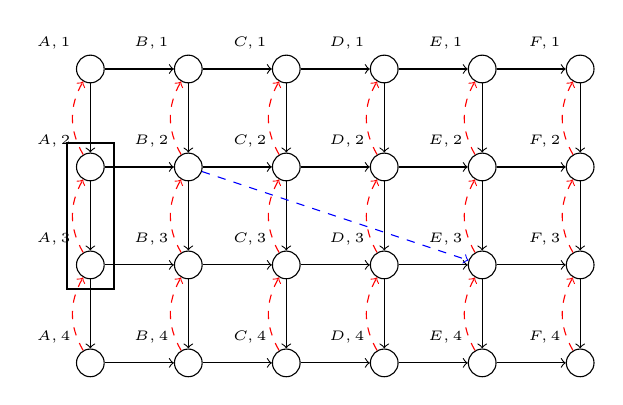
\begin{tikzpicture}[operation/.style={circle,draw=black, fill=white,inner sep=0pt, minimum size=1.0em},
    cluster/.style={shape=ellipse,draw},
    every node/.style={node distance=2.5em}
    ]
    \def\jobs{A,B,C,D, E, F}
    \def\operations{1,2,3,4}
    
    \def\prevx{A}
    \message{Start}
    \foreach \x[count=\xi from 0, remember=\x as \prevx] in \jobs {
        \def\prevy{}
        \foreach \y[count=\yi from 0, remember=\y as \prevy] in \operations {
            \def\nodename{\tiny ${\x,\y}$}
            % draw the operations for this job
            \ifnum \yi = 0
            \ifnum \xi = 0
            \node[operation, label=above left:\nodename] (\x\y) {};
            \else 
            \node[operation, label=above left:\nodename, right=of \prevx\y] (\x\y) {};
            \fi
            \else 
            \node[operation, below=of \x\prevy, label=above left:\nodename] (\x\y) {};
            % add downward arrow, from previous operation
            \ifnum \yi > 0
            \path[every edge/.style={draw}, ->] 
            (\x\prevy) edge (\x\y);
            \path[every edge/.style={draw=red, dashed}, ->]
            (\x\y) edge [bend left] (\x\prevy);                        
            \fi
            \fi
            
            \ifnum \xi > 0
            % draw arrows from last to current
            \path[every edge/.style={draw}, ->]
            (\prevx\y) edge (\x\y);
            \fi
        }
    }
    
    \node[fit=(A2)(\prevx 3), line width=0.75pt, draw] {};
    
    \path[every edge/.style={draw=blue, dashed}, ->]
    (B2) edge (E3)
    ;
    
    \end{tikzpicture}
    \caption{Example of a non-ordering dependency that might unnecessarily restrict the starting times of operation E3 and further.
        %            Would be nice to show which ASAP times can never be influenced anymore after fixing this ordering tuple! Show in case of forward iteration. Also, maybe make this a foreach(a,b,c,d) script?
    }
    \label{fig:example_non_ordering}
\end{figure}

\section{Properties of the (2-)re-entrant flowshop}
Take as example the 3 machine flow shop $F_{3,<1,2,1>}$ where the second machine is 2-re-entrant. This flowshop is used to model the printer case. Operation $x$ of job $j$ is denoted with $O_{j,x}$. When there is a direct precedence relationship from $O_{j,x}$ to $O_{k,y}$, then we denote this with $O_{j,x} \to O_{k,y}$. When there is a (transitive) precedence relationship from $O_{j,x}$ to $O_{k,y}$, then we denote this with $O_{j,x} \prec O_{k,y}$.

Firstly, the problem definition states that the sequence of jobs (i.e. sheet) is totally ordered:
\begin{equation}
\forall O_{i,x}, O_{j,x} \in F | i < j : O_{i,x} \prec O_{j,x}
\end{equation}

Secondly, the operations in a job are also totally ordered:

\begin{equation}
\forall O_{j,x}, O_{j,x+1} \in F : O_{j,x} \to O_{j,x+1}
\end{equation}

A valid schedule is found by creating a \textit{feasible total ordering} of the operations on the re-entrant machine(s). Note that the operations of non-re-entrant machines do not need to be scheduled as their operations are totally ordered by definition.
\begin{figure}
    \centering
    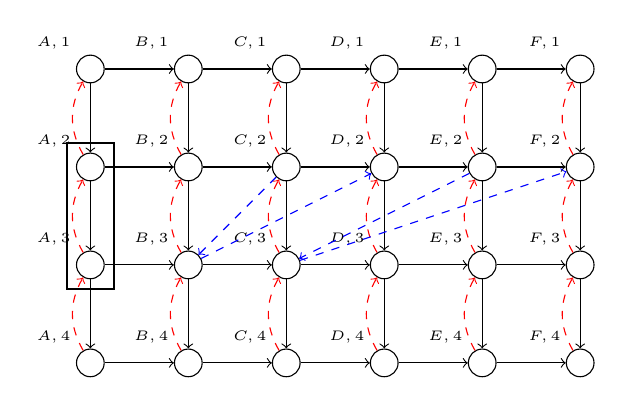
\begin{tikzpicture}[operation/.style={circle,draw=black, fill=white,inner sep=0pt, minimum size=1.0em},
    cluster/.style={shape=ellipse,draw},
    every node/.style={node distance=2.5em}
    ]
    \def\jobs{A,B,C,D, E, F}
    \def\operations{1,2,3,4}
    
    \def\prevx{A}
    \message{Start}
    \foreach \x[count=\xi from 0, remember=\x as \prevx] in \jobs {
        \def\prevy{}
        \foreach \y[count=\yi from 0, remember=\y as \prevy] in \operations {
            \def\nodename{\tiny ${\x,\y}$}
            % draw the operations for this job
            \ifnum \yi = 0
            \ifnum \xi = 0
            \node[operation, label=above left:\nodename] (\x\y) {};
            \else 
            \node[operation, label=above left:\nodename, right=of \prevx\y] (\x\y) {};
            \fi
            \else 
            \node[operation, below=of \x\prevy, label=above left:\nodename] (\x\y) {};
            % add downward arrow, from previous operation
            \ifnum \yi > 0
            \path[every edge/.style={draw}, ->] 
            (\x\prevy) edge (\x\y);
            \path[every edge/.style={draw=red, dashed}, ->]
            (\x\y) edge [bend left] (\x\prevy);                        
            \fi
            \fi
            
            \ifnum \xi > 0
            % draw arrows from last to current
            \path[every edge/.style={draw}, ->]
            (\prevx\y) edge (\x\y);
            \fi
        }
    }
    
    \node[fit=(A2)(\prevx 3), line width=0.75pt, draw] {};
    
    \path[every edge/.style={draw=blue, dashed}, ->]
    (C2) edge (B3)
    (B3) edge (D2)
    ;
    
    \path[every edge/.style={draw=blue, dashed}, ->]
    (E2) edge (C3)
    (C3) edge (F2)
    ;
    
    
    \end{tikzpicture}
    \caption{Second pass of job 2 can be interleaved between first pass of job 3 and 4 if the deadline between first and second pass of job allows that; dashed red edges are deadlines (and are modelled with negative weights), the ordering tuple is shown with dashed blue edges.
        %            Would be nice to show which ASAP times can never be influenced anymore after fixing this ordering tuple! Show in case of forward iteration. Also, maybe make this a foreach(a,b,c,d) script?
    }
    \label{fig:example_flowshop_scheduling_ordering_tuple}
\end{figure}

Although in the generic case the deadlines can be defined between arbitrary operations, there is typically a certain structure to the deadlines and setup times in the flow shop. In the printer case, for example, the deadlines are all intra-job deadlines: i.e. in Figure~\ref{fig:example_flowshop_scheduling_ordering_tuple} the source and destination of the dashed red edges are all from the same job. This enables us to use invariants to reduce the total complexity of the graph structure.

An ordering tuple is a tuple $(a,b,c)$ which takes 3 operations and imposes a sequential constraint, eliminating possible parallelism: $a \prec b \prec c$, and $a\to c$. The analogy of the ordering tuple in the printer case is interleaving second-pass sheets with first-pass sheets. 

Resolving the re-entrancy is done by selecting which \textit{ordering tuple} is the most productive, while not sacrificing too much flexibility\footnote{leaving in the middle whether you use a ranking or trade-off scheduler}. Such ordering tuples are generated for each combination of possible interleaving. I.e. for each job, it considers whether a higher-pass operation can be inserted in between two directly adjacent lower-pass operations. 

\subsection{Purging infeasible combinations of ordering tuples}
The higher-pass operation is necessarily of an earlier job than the current job being scheduled (as the jobs and operations per job are totally ordered). Given two ordering tuples $(a,b,c)$ and $(d,e,f)$ where $c\preceq d$, the combination of the two is definitely infeasible when:
\begin{equation}
\forall (a,b,c), (d,e,f) \in OT : e \prec b
\end{equation}
as a a positive cycle over $b \prec c \preceq d \prec e \prec b$ would necessarily exist\footnote{under the assumption that operations always take a positive non-zero amount of time; it might not hold under 3-re-entrancy either} since:
\begin{equation}
\begin{rcases}
    a \prec b \prec c\\
    c \preceq d\\
    d \prec e \prec f\\
    e \prec b
\end{rcases} b \prec c \preceq d \prec e \prec b
\end{equation}
See for an example Figure~\ref{fig:example_flowshop_scheduling_ordering_tuple_positive_cycle}.

{\large \bfseries Remark: can we generalize this also to higher re-entrancy than 2-re-entrancy?}
\begin{figure}
    \centering
    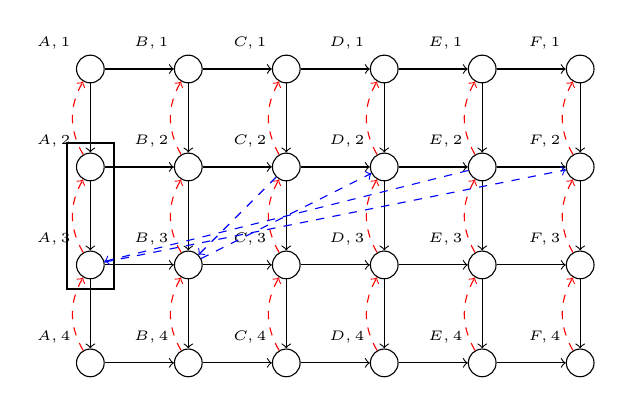
\begin{tikzpicture}[operation/.style={circle,draw=black, fill=white,inner sep=0pt, minimum size=1.0em},
    cluster/.style={shape=ellipse,draw},
    every node/.style={node distance=2.5em}
    ]
    \def\jobs{A,B,C,D, E, F}
    \def\operations{1,2,3,4}
    
    \def\prevx{A}
    \message{Start}
    \foreach \x[count=\xi from 0, remember=\x as \prevx] in \jobs {
        \def\prevy{}
        \foreach \y[count=\yi from 0, remember=\y as \prevy] in \operations {
            \def\nodename{\tiny ${\x,\y}$}
            % draw the operations for this job
            \ifnum \yi = 0
            \ifnum \xi = 0
            \node[operation, label=above left:\nodename] (\x\y) {};
            \else 
            \node[operation, label=above left:\nodename, right=of \prevx\y] (\x\y) {};
            \fi
            \else 
            \node[operation, below=of \x\prevy, label=above left:\nodename] (\x\y) {};
            % add downward arrow, from previous operation
            \ifnum \yi > 0
            \path[every edge/.style={draw}, ->] 
            (\x\prevy) edge (\x\y);
            \path[every edge/.style={draw=red, dashed}, ->]
            (\x\y) edge [bend left] (\x\prevy);                        
            \fi
            \fi
            
            \ifnum \xi > 0
            % draw arrows from last to current
            \path[every edge/.style={draw}, ->]
            (\prevx\y) edge (\x\y);
            \fi
        }
    }
    
    \node[fit=(A2)(\prevx 3), line width=0.75pt, draw] {};
    
    \path[every edge/.style={draw=blue, dashed}, ->]
    (C2) edge (B3)
    (B3) edge (D2)
    ;
    
    \path[every edge/.style={draw=blue, dashed}, ->]
    (E2) edge (A3)
    (A3) edge (F2)
    ;
    
    
    \end{tikzpicture}
    \caption{Infeasible combination of ordering tuples: a positive cycle exists: $B,3 \to D,2 \to E,2 \to A, 3 \to B,3$ }
    \label{fig:example_flowshop_scheduling_ordering_tuple_positive_cycle}
\end{figure}
\subsection{Purging ordering tuples with infeasible deadlines}
The intra-job deadlines of the printer case can be leveraged to purge the combinations. Take an ordering tuple $(a,b,c)$ where there $\exists b' : b' \to \wedge b' \prec a$. The lower bound on the time between $b'$ and $a$ gives a hint to the maximal slack on the deadline. If this slack is negative, then the graph contains a positive cycle. The minimum time between $b'$ and $a$ is the sum of operations between them. This may be calculated by using a longest path algorithm from $b'$ to $a$, or by using only the sum of operations in a certain path between $b'$ and $a$ \footnote{we may be able to prove that it's always a certain path, and the generic shortest path might be overkill to use}. Once an ordering tuple $(a,b,c)$ has been deemed infeasible, any ordering tuple $(d,e,f)$ with $a \prec d$ has necessarily less slack on the deadline, and is therefore also infeasible.

\begin{figure}
    \centering
    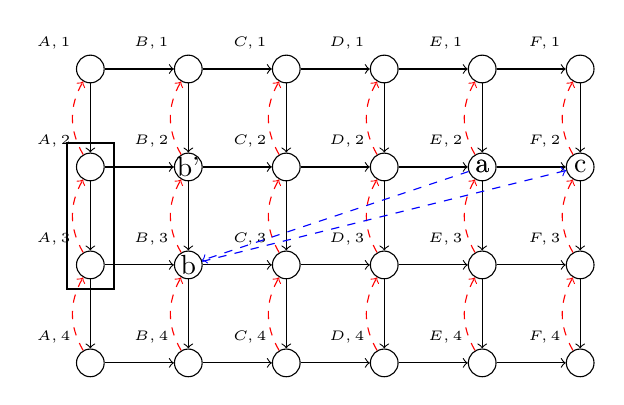
\begin{tikzpicture}[operation/.style={circle,draw=black, fill=white,inner sep=0pt, minimum size=1.0em},
        cluster/.style={shape=ellipse,draw},
        every node/.style={node distance=2.5em}
        ]
        \def\jobs{A,B,C,D, E, F}
        \def\operations{1,2,3,4}
        
        \def\prevx{A}
        \message{Start}
        \foreach \x[count=\xi from 0, remember=\x as \prevx] in \jobs {
        \def\prevy{}
        \foreach \y[count=\yi from 0, remember=\y as \prevy] in \operations {
            \def\nodename{\tiny ${\x,\y}$}
            % draw the operations for this job
            \ifnum \yi = 0
            \ifnum \xi = 0
            \node[operation, label=above left:\nodename] (\x\y) {};
            \else 
            \node[operation, label=above left:\nodename, right=of \prevx\y] (\x\y) {};
            \fi
            \else 
            \node[operation, below=of \x\prevy, label=above left:\nodename] (\x\y) {};
            % add downward arrow, from previous operation
            \ifnum \yi > 0
            \path[every edge/.style={draw}, ->] 
            (\x\prevy) edge (\x\y);
            \path[every edge/.style={draw=red, dashed}, ->]
            (\x\y) edge [bend left] (\x\prevy);                        
            \fi
            \fi
            
            \ifnum \xi > 0
            % draw arrows from last to current
            \path[every edge/.style={draw}, ->]
            (\prevx\y) edge (\x\y);
            \fi
        }
    }
    
    \node[fit=(A2)(\prevx 3), line width=0.75pt, draw] {};

    \path[every edge/.style={draw=blue, dashed}, ->]
    (E2) edge  (B3) node {a}
    (B3) edge (F2)
    ;
    % nasty part to add labels to existing nodes...
    \path 
        (E2) edge (E2) node {a}
        (B3) edge (B3) node {b}	
        (F2) edge (F2) node {c}
        (B2) edge (B2) node {b'}        
    ;
    
    \end{tikzpicture}
    \caption{The ordering tuple (a,b,c) may never be able to meet the deadline between B,3 and B,2}
    \label{fig:example_flowshop_infeasible_deadline_tuple}
\end{figure}

\section{Windowing}
From here on out, we assume that the re-entrancy is resolved per operation, from the first job to the last job, or vice-versa.

We have shown two mechanisms that can be leveraged to limit the calculation of interactions between starting-times. One provides a starting point (i.e. lower bound) for the window, and the other provides an upper bound.

The lower bound is determined by the \textit{last interleaved operation}. It determines that no operation preceding the last interleaved can be regarded as a feasible scheduling option anymore, as it would introduce a positive cycle (i.e. infeasibility) in the graph. I.e., imposing both $O_{k, x} \prec O_{l, x+1}$ and $O_{l, x} \prec O_{j, x+1}$ (when $j < k < l$). 

This means that, after some point, the deadline of an interleaved higher pass is already passed. I.e. any ordering tuple after that operation, can never lead to a feasible interleaving, as operation times are non-negative.

The upper bound is determined by the deadline constraint between the current operation under consideration, and the minimal setup + operation times of the following operations. 

These two heuristics lead to the extraction of a natural window, if one exists. Using said window may help greatly to avoid most of the expensive calls. Of course, this only helps if $W \ll V$ indeed holds. For small $V$ it might not, but it will help in typical cases where the jobs are large.

\section{Bellman-Ford implementations}

The Bellman-Ford algorithm determines an upper bound on the number of (useful) relaxations that need to be done on the graph. It detects infeasibility in case after that upper bound there are still changes observed when relaxing the edges. Any implementation of Bellman-Ford needs to ensure that it will relax the longest possible path, and that it can detect the existence negative cycles.

The simplest Bellman-Ford implementation is the following algorithm:

\begin{algorithm}
\caption{Original BellmanFordSP}    
\begin{algorithmic}[H]
    \Function{BellmanFordSP}{Graph $G(V,E, w)$, source $s \in V$}
    \ForAll{vertices $u \in V(G)$}
        \State $d(u) = \infty$
    \EndFor
    \State $d(s) = 0$\\
    \State \Comment{Compute the shortest paths by relaxing all edges $|V(G)|$ times}
    \For{$|V(G)|-1$}
        \ForAll{edges $u,v \in E(G)$}
            \State \Call{Relax}{u,v,w}
        \EndFor
    \EndFor\\
    \State \Comment{Detect existence of negative cycles}
    \State feasible = true
    \ForAll{edges $u,v \in E(G)$}
        \State feasible = feasible and not \Call{Relax}{u,v,w}
    \EndFor\\
    \State \Return feasible, $d$
    \EndFunction
%\caption{Basic implementation of Bellman-Ford}
\end{algorithmic}
\end{algorithm}

\begin{algorithm}
  \caption{Relax one edge: return true when edge has been relaxed, false otherwise}
\begin{algorithmic}[H]
    \Function{Relax}{$u,v,w$}
    \If{$d(u) + w < d(v)$}
        \State $d(v) = d(u) + w$
        \State \Return true
    \EndIf
    \State \Return false
    
    \EndFunction
    %\caption{Basic implementation of Bellman-Ford}
\end{algorithmic}
\end{algorithm}


The queue-implementation~\cite{books/daglib/0029345} \cite{BellmanFordOnGPUKepler}, which considers the active vertices:

\begin{algorithm}
    \caption{BellmanFordSP-queue}    
    \begin{algorithmic}[H]
        \Function{BellmanFord-Queue}{Graph $G(V,E, w)$, source $s \in V$}
        \ForEach{vertices $u \in V(G)$}
        \State $d(u) = \infty$
        \State $l(u) = 0$
        \EndFor
        \State $d(s) = 0$\\
        \State \Comment{Compute the shortest paths by relaxing edges from eligible vertices}
        \State F = \{s\}
        
        \State feasible = true
        \While{$F \neq \emptyset$ and feasible}
            \State pick $v \in F$
            \State $F = F / v$
            \State feasible = feasible $\wedge$ \Call{Relax-queue}{$v$}
        \EndWhile

        \State \Return feasible, $d$
        \EndFunction
    \end{algorithmic}
\end{algorithm}

\begin{algorithm}
    \caption{Relax one vertex: return true when considered feasible, false when infeasible}
    \begin{algorithmic}[H]
        \Function{Relax-queue}{$v$}
        \ForEach{$s,t \in out(v)$}
        \If{$d(s) + w < d(t)$}
        \State $d(t) = d(s) + w$
        \State $F = F \cup {t}$ \Comment{Mark target as eligible for relaxation}
        \State $l(t) = l(s) + 1$ \Comment{Shortest path is found from here}
        \State \Comment{If the relaxation path covers more than $|V(G)|$ vertices, a negative cycle must exist}
        \State \Return $l(t) < |V(G)|$ 
        \EndIf
        \Return true \Comment{not relaxed, no reason that this is suddenly infeasible}
        \EndFor
        
        \EndFunction
        %\caption{Basic implementation of Bellman-Ford}
    \end{algorithmic}
\end{algorithm}

\section{Finite horizon Bellman-Ford}

Consider forward iteration\footnote{For reverse iteration this becomes much more convoluted, as the incoming paths may change and therefore everything may need to be re-computed}, where the Bellman-Ford algorithm has calculated starting times for the previous schedule. Anything scheduled before the last interleaved operation are not allowed to be re-timed anymore; their ASAP-times become fixed, and don't need to be re-calculated. We can use the first operation of the job which contains the interleaved operation as source and the rest of the algorithm can remain the same.

It is possible that a scheduling choice pushes the second pass sheet to a later starting time. As the deadline imposed on the second pass sheets may mean it needs to schedule its corresponding first pass later than planned, this may again have impact on the second pass of an even earlier sheet. If this earlier sheet has enough slack on its deadline, \'and the setup time between those operations does not exceed the sum of the processing times and setup times between the first passes of the sheets, then the schedule will be stable and feasible. As the deadlines for second pass sheets can delay their corresponding first pass transitively, the extent of a scheduling decision may encompass re-timing all operations to detect that it is a feasible decision.

Figure~\ref{fig:example_flowshop_recursive_backpressure} shows an example where a set-up time between the first pass of A and second pass B may lead to a later starting time than the first pass of B. This in turn may lead to later second passes of previous jobs, which in turn can propagate to their corresponding first pass. We therefore cannot guarantee that future scheduling decisions will not influence operations that are not local to the decision. This makes it impossible to determine a window in which the influence of scheduling decisions on previously calculated starting times are all captured. However, we can take the penalty of not re-timing the operations outside the window.

In the Oc\'e case this implies that we do not make full use of the buffer; it only works when we determine up front that the buffer will be large enough to accommodate a scheduling decision productively.

\begin{figure}
    \centering
    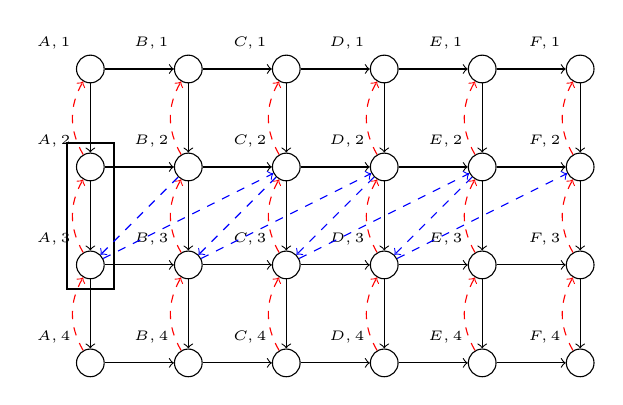
\begin{tikzpicture}[operation/.style={circle,draw=black, fill=white,inner sep=0pt, minimum size=1.0em},
    cluster/.style={shape=ellipse,draw},
    every node/.style={node distance=2.5em}
    ]
    \def\jobs{A,B,C,D, E, F}
    \def\operations{1,2,3,4}
    
    \def\prevx{A}
    \message{Start}
    \foreach \x[count=\xi from 0, remember=\x as \prevx] in \jobs {
        \def\prevy{}
        \foreach \y[count=\yi from 0, remember=\y as \prevy] in \operations {
            \def\nodename{\tiny ${\x,\y}$}
            % draw the operations for this job
            \ifnum \yi = 0
            \ifnum \xi = 0
            \node[operation, label=above left:\nodename] (\x\y) {};
            \else 
            \node[operation, label=above left:\nodename, right=of \prevx\y] (\x\y) {};
            \fi
            \else 
            \node[operation, below=of \x\prevy, label=above left:\nodename] (\x\y) {};
            % add downward arrow, from previous operation
            \ifnum \yi > 0
            \path[every edge/.style={draw}, ->] 
            (\x\prevy) edge (\x\y);
            \path[every edge/.style={draw=red, dashed}, ->]
            (\x\y) edge [bend left] (\x\prevy);                        
            \fi
            \fi
            
            \ifnum \xi > 0
            % draw arrows from last to current
            \path[every edge/.style={draw}, ->]
            (\prevx\y) edge (\x\y);
            \fi
        }
    }
    
    \node[fit=(A2)(\prevx 3), line width=0.75pt, draw] {};
    
    \path[every edge/.style={draw=blue, dashed}, ->]
        (B2) edge  (A3)
        (A3) edge (C2)
        
        (C2) edge  (B3)
        (B3) edge (D2)
        
        (D2) edge  (C3)
        (C3) edge (E2) 
        
        (E2) edge  (D3)
        (D3) edge (F2)                     
    ;
    % nasty part to add labels to existing nodes...
%    \path 
%    (E2) edge (E2) node {a}
%    (B3) edge (B3) node {b}	
%    (F2) edge (F2) node {c}
%    (B2) edge (B2) node {b'}        
%    ;
    
    \end{tikzpicture}
    \caption{The 'backpressure' on the edges imposed by the deadlines and the interleaving decisions may lead to later start-times than without the choice. There seems to be no general way to determine how far back it can propagate.}
    \label{fig:example_flowshop_recursive_backpressure}
\end{figure}

However, as we know that there is a limited window of opportunity, we can take this information into account as well; any calculation that involves starting from any of the nodes outside of that window don't need to be taken into account either, as they do not yet impose additional constraints on the starting times\footnote{although the Bellman-Ford algorithm may not see this immediately, we just don't need to consider that information yet, and can simply skip calculating it}.

To tighten the worst-case complexity from $O(W \cdot E)$ to $O(W^2)$, we need to show that the edge set involving nodes from $W$ is equal to at most $6\cdot (r-1) + 4 \cdot (|J| - 1) + 2$, and $|J|$ has been limited to $|W|$, as the jobs before the window have already been fixed.

Remark: to implement this needs some further investigation; e.g. copying around all the ASAP times all the time is not very efficient.

\section{Transitive reduction of the scheduling decisions}

The constraint graph encodes the requirements that e.g. $x_2 \geq x_1 + \alpha$, which is denoted by an edge with weight $\alpha$ from $x_1$ to $x_2$, as shown in Figure~\ref{fig:transitive_closure_simple_example}.

An illustration shows how this could be applied. With the system of inequalities that need to be satisfied given as:

\begin{align*}
\begin{pmatrix}
x_3 \geq x1 + \alpha\\
x_2 \geq x1 + \beta\\
x_3 \geq x2 + \gamma\\
\end{pmatrix}
\equiv
\begin{pmatrix}
x_2 \geq x1 + \beta\\
x_3 \geq \max{\left(x2 + \gamma, x1 + \alpha\right)}\\
\end{pmatrix}
\\
\equiv
\begin{pmatrix}
x_2 \geq x1 + \beta\\
x_3 \geq x1 + \max{\left(\beta + \gamma, \alpha\right)}\\
\end{pmatrix}
\equiv
\begin{pmatrix}
x_2 \geq x1 + \beta\\
x_3 \geq x2 + \max{\left(\gamma, \alpha - \beta\right)}\\
\end{pmatrix}
\end{align*}

The last set of inequalities is also visualized in Figure~\ref{fig:transitive_closure_simple_example_reduced}. We use this transitive reduction method to reduce the scheduling decisions shown in Figure~\ref{fig:transitive_closure_simple_example} into Figure~\ref{fig:transitive_closure_simple_example_reduced}.

Generically, the trapezoid 

\begin{figure}
    \centering
    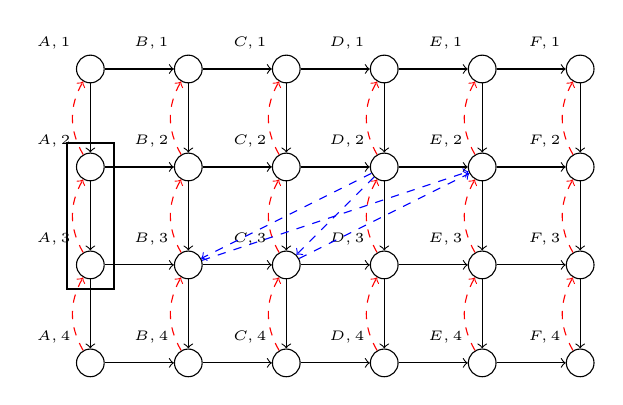
\begin{tikzpicture}[operation/.style={circle,draw=black, fill=white,inner sep=0pt, minimum size=1.0em},
    cluster/.style={shape=ellipse,draw},
    every node/.style={node distance=2.5em}
    ]
    \def\jobs{A,B,C,D, E, F}
    \def\operations{1,2,3,4}
    
    \def\prevx{A}
    \message{Start}
    \foreach \x[count=\xi from 0, remember=\x as \prevx] in \jobs {
        \def\prevy{}
        \foreach \y[count=\yi from 0, remember=\y as \prevy] in \operations {
            \def\nodename{\tiny ${\x,\y}$}
            % draw the operations for this job
            \ifnum \yi = 0
            \ifnum \xi = 0
            \node[operation, label=above left:\nodename] (\x\y) {};
            \else 
            \node[operation, label=above left:\nodename, right=of \prevx\y] (\x\y) {};
            \fi
            \else 
            \node[operation, below=of \x\prevy, label=above left:\nodename] (\x\y) {};
            % add downward arrow, from previous operation
            \ifnum \yi > 0
            \path[every edge/.style={draw}, ->] 
            (\x\prevy) edge (\x\y);
            \path[every edge/.style={draw=red, dashed}, ->]
            (\x\y) edge [bend left] (\x\prevy);                        
            \fi
            \fi
            
            \ifnum \xi > 0
            % draw arrows from last to current
            \path[every edge/.style={draw}, ->]
            (\prevx\y) edge (\x\y);
            \fi
        }
    }
    
    \node[fit=(A2)(\prevx 3), line width=0.75pt, draw] {};
    
    \path[every edge/.style={draw=blue, dashed}, ->]
    (D2) edge  (B3)
    (B3) edge (E2)
    (D2) edge  (C3)
    (C3) edge (E2)
    ;
    
    \end{tikzpicture}
    \caption{Example of scheduling decisions that can be reduced}
    \label{fig:example_flowshop_reducable_interleavings}
\end{figure}

\begin{figure}
    \centering
    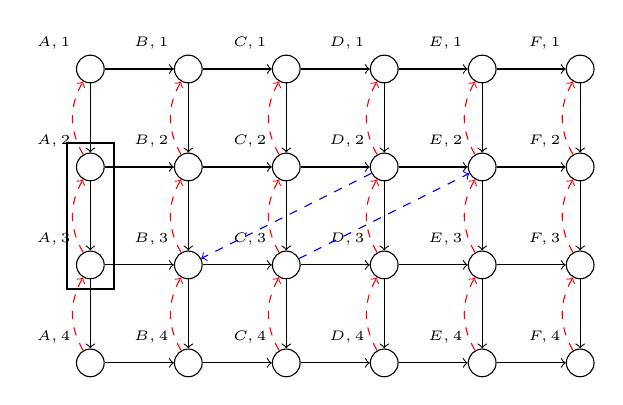
\begin{tikzpicture}[operation/.style={circle,draw=black, fill=white,inner sep=0pt, minimum size=1.0em},
    cluster/.style={shape=ellipse,draw},
    every node/.style={node distance=2.5em}
    ]
    \def\jobs{A,B,C,D, E, F}
    \def\operations{1,2,3,4}
    
    \def\prevx{A}
    \message{Start}
    \foreach \x[count=\xi from 0, remember=\x as \prevx] in \jobs {
        \def\prevy{}
        \foreach \y[count=\yi from 0, remember=\y as \prevy] in \operations {
            \def\nodename{\tiny ${\x,\y}$}
            % draw the operations for this job
            \ifnum \yi = 0
            \ifnum \xi = 0
            \node[operation, label=above left:\nodename] (\x\y) {};
            \else 
            \node[operation, label=above left:\nodename, right=of \prevx\y] (\x\y) {};
            \fi
            \else 
            \node[operation, below=of \x\prevy, label=above left:\nodename] (\x\y) {};
            % add downward arrow, from previous operation
            \ifnum \yi > 0
            \path[every edge/.style={draw}, ->] 
            (\x\prevy) edge (\x\y);
            \path[every edge/.style={draw=red, dashed}, ->]
            (\x\y) edge [bend left] (\x\prevy);                        
            \fi
            \fi
            
            \ifnum \xi > 0
            % draw arrows from last to current
            \path[every edge/.style={draw}, ->]
            (\prevx\y) edge (\x\y);
            \fi
        }
    }
    
    \node[fit=(A2)(\prevx 3), line width=0.75pt, draw] {};
    
    \path[every edge/.style={draw=blue, dashed}, ->]
    (D2) edge  (B3)
    (C3) edge (E2)
    ;
    
    \end{tikzpicture}
    \caption{Example reduced set of scheduling decisions }
    \label{fig:example_flowshop_reduced_interleavings}
\end{figure}
\begin{figure}
    \centering
    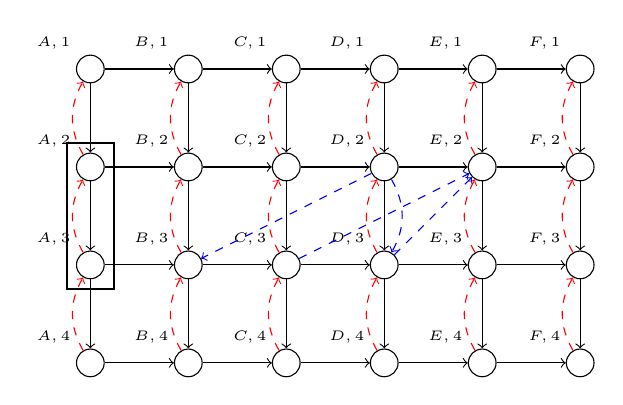
\begin{tikzpicture}[operation/.style={circle,draw=black, fill=white,inner sep=0pt, minimum size=1.0em},
    cluster/.style={shape=ellipse,draw},
    every node/.style={node distance=2.5em}
    ]
    \def\jobs{A,B,C,D, E, F}
    \def\operations{1,2,3,4}
    
    \def\prevx{A}
    \message{Start}
    \foreach \x[count=\xi from 0, remember=\x as \prevx] in \jobs {
        \def\prevy{}
        \foreach \y[count=\yi from 0, remember=\y as \prevy] in \operations {
            \def\nodename{\tiny ${\x,\y}$}
            % draw the operations for this job
            \ifnum \yi = 0
            \ifnum \xi = 0
            \node[operation, label=above left:\nodename] (\x\y) {};
            \else 
            \node[operation, label=above left:\nodename, right=of \prevx\y] (\x\y) {};
            \fi
            \else 
            \node[operation, below=of \x\prevy, label=above left:\nodename] (\x\y) {};
            % add downward arrow, from previous operation
            \ifnum \yi > 0
            \path[every edge/.style={draw}, ->] 
            (\x\prevy) edge (\x\y);
            \path[every edge/.style={draw=red, dashed}, ->]
            (\x\y) edge [bend left] (\x\prevy);                        
            \fi
            \fi
            
            \ifnum \xi > 0
            % draw arrows from last to current
            \path[every edge/.style={draw}, ->]
            (\prevx\y) edge (\x\y);
            \fi
        }
    }
    
    \node[fit=(A2)(\prevx 3), line width=0.75pt, draw] {};
    
    \path[every edge/.style={draw=blue, dashed}, ->]
    (D2) edge  (B3)
    (C3) edge (E2)
    (D2) edge[bend left] (D3)
    (D3) edge (E2)
    ;
    
    \end{tikzpicture}
    \caption{Example reduced set of scheduling decisions}
    \label{fig:example_flowshop_reduced_interleavings_more}
\end{figure}
\begin{figure}
    \centering
    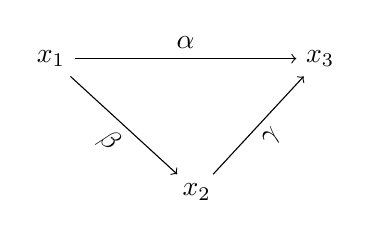
\begin{tikzpicture}
        \node (A) {$x_1$};
        \node[right=8em of A](B) {$x_3$};
        \node[below right=5em of A] (C) {$x_2$};
        \path[->]
            (A) edge node[above, midway, sloped] {$\alpha$} (B)
            (A) edge node[below, midway, sloped] {$\beta$} (C)  
            (C) edge node[below, midway, sloped] {$\gamma$} (B);
    \end{tikzpicture}
    \caption{Simple example for the transitive closure}
    \label{fig:transitive_closure_simple_example}

    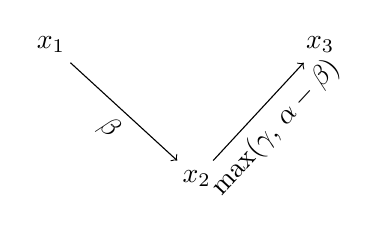
\begin{tikzpicture}
        \node (A) {$x_1$};
        \node[right=8em of A](B) {$x_3$};
        \node[below right=5em of A] (C) {$x_2$};
        \path[->]
            (A) edge node[below, midway, sloped] {$\beta$} (C)  
            (C) edge node[below, midway, sloped] {max($\gamma$, $\alpha - \beta$)} (B);
    \end{tikzpicture}
    \caption{Reduced version of the simple example}
    \label{fig:transitive_closure_simple_example_reduced}

\end{figure}

\begin{figure}
    \centering
    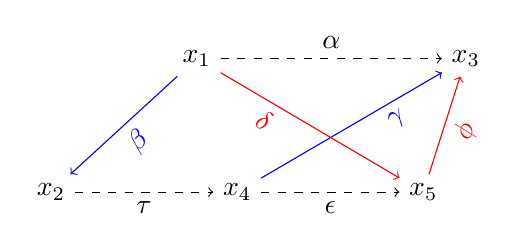
\begin{tikzpicture}
    \node (A) {$x_1$};
    \node[right=8em of A](B) {$x_3$};
    \node[below left=5em of A] (C) {$x_2$};
    \node[right=5em of C] (D) {$x_4$};
    \node[right=5em of D] (E) {$x_5$};
    \path[->]
    (A) edge[blue] node[below, midway, sloped] {$\beta$} (C)  
    (D) edge[blue] node[below, pos=0.7, sloped] {$\gamma$} (B)
    (A) edge[red] node[below, pos=0.3, sloped] {$\delta$} (E)
    (E) edge[red] node[below, midway, sloped] {$\phi$} (B)
    ;

    \path[every edge/.style={draw, dashed}, ->] 
    (A) edge node[above, midway, sloped] {$\alpha$} (B)
    (C) edge node[below, midway, sloped] {$\tau$} (D)
    (D) edge node[below, midway, sloped] {$\epsilon$} (E)
    ;
    \end{tikzpicture}
    \caption{4-node example for the transitive closure}
    \label{fig:transitive_closure_4_node_example}
    
    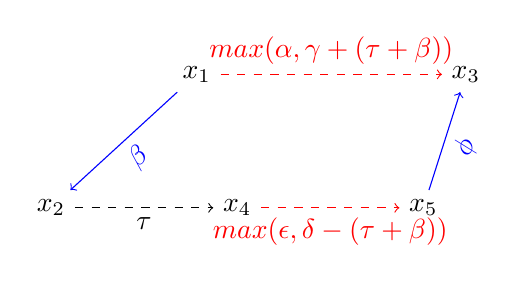
\begin{tikzpicture}
    \node (A) {$x_1$};
    \node[right=8em of A](B) {$x_3$};
    \node[below left=5em of A] (C) {$x_2$};
    \node[right=5em of C] (D) {$x_4$};
    \node[right=5em of D] (E) {$x_5$};
    \path[->]
    (A) edge[blue] node[below, midway, sloped] {$\beta$} (C)  
    (E) edge[blue] node[below, midway, sloped] {$\phi$} (B)
    ;
    
    \path[every edge/.style={draw, dashed}, ->] 
    (A) edge[red] node[above, midway, sloped] {$max(\alpha, \gamma + (\tau + \beta))$} (B)
    (C) edge node[below, midway, sloped] {$\tau$} (D)
    (D) edge[red] node[below, midway, sloped] {$max(\epsilon, \delta -(\tau+\beta))$} (E)
    ;
    \end{tikzpicture}
    \caption{Reduced version of the 4-node example}
    \label{fig:transitive_closure_4_node_example_reduced}
    
\end{figure}

\section{Other remarks}
In definition 8 from Umar's DATE paper the requirement for feasibility is necessary, but not (by definition?) sufficient. On arbitrary graphs, the \textit{feasibility of a schedule} may be compromised by a \textit{feasible choice}, as it may lead to infeasibility of all other choices later on. This may be caused by (strangely structured) setup times and deadlines? It is of no concern in the Oc\'e case.

It might also be better to resolve the re-entrancy of one job first, as that may lead to fewer infeasible schedules later. The idea is that the first ordering tuple can lead to high amounts of 'stress' on the deadline of later re-entrancies, which can then not be resolved to previous scheduling decisions.

% Bibliography.
\bibliographystyle{abbrv}
\bibliography{references}

\end{document}
